\documentclass[handout]{ximera}
\usepackage{gensymb}
\usepackage{tabularx}
\usepackage{mdframed}
\usepackage{pdfpages}
%\usepackage{chngcntr}

\let\problem\relax
\let\endproblem\relax

\newcommand{\property}[2]{#1#2}




\newtheoremstyle{SlantTheorem}{\topsep}{\fill}%%% space between body and thm
 {\slshape}                      %%% Thm body font
 {}                              %%% Indent amount (empty = no indent)
 {\bfseries\sffamily}            %%% Thm head font
 {}                              %%% Punctuation after thm head
 {3ex}                           %%% Space after thm head
 {\thmname{#1}\thmnumber{ #2}\thmnote{ \bfseries(#3)}} %%% Thm head spec
\theoremstyle{SlantTheorem}
\newtheorem{problem}{Problem}[]

%\counterwithin*{problem}{section}



%%%%%%%%%%%%%%%%%%%%%%%%%%%%Jenny's code%%%%%%%%%%%%%%%%%%%%

%%% Solution environment
%\newenvironment{solution}{
%\ifhandout\setbox0\vbox\bgroup\else
%\begin{trivlist}\item[\hskip \labelsep\small\itshape\bfseries Solution\hspace{2ex}]
%\par\noindent\upshape\small
%\fi}
%{\ifhandout\egroup\else
%\end{trivlist}
%\fi}
%
%
%%% instructorIntro environment
%\ifhandout
%\newenvironment{instructorIntro}[1][false]%
%{%
%\def\givenatend{\boolean{#1}}\ifthenelse{\boolean{#1}}{\begin{trivlist}\item}{\setbox0\vbox\bgroup}{}
%}
%{%
%\ifthenelse{\givenatend}{\end{trivlist}}{\egroup}{}
%}
%\else
%\newenvironment{instructorIntro}[1][false]%
%{%
%  \ifthenelse{\boolean{#1}}{\begin{trivlist}\item[\hskip \labelsep\bfseries Instructor Notes:\hspace{2ex}]}
%{\begin{trivlist}\item[\hskip \labelsep\bfseries Instructor Notes:\hspace{2ex}]}
%{}
%}
%% %% line at the bottom} 
%{\end{trivlist}\par\addvspace{.5ex}\nobreak\noindent\hung} 
%\fi
%
%


\let\instructorNotes\relax
\let\endinstructorNotes\relax
%%% instructorNotes environment
\ifhandout
\newenvironment{instructorNotes}[1][false]%
{%
\def\givenatend{\boolean{#1}}\ifthenelse{\boolean{#1}}{\begin{trivlist}\item}{\setbox0\vbox\bgroup}{}
}
{%
\ifthenelse{\givenatend}{\end{trivlist}}{\egroup}{}
}
\else
\newenvironment{instructorNotes}[1][false]%
{%
  \ifthenelse{\boolean{#1}}{\begin{trivlist}\item[\hskip \labelsep\bfseries {\Large Instructor Notes: \\} \hspace{\textwidth} ]}
{\begin{trivlist}\item[\hskip \labelsep\bfseries {\Large Instructor Notes: \\} \hspace{\textwidth} ]}
{}
}
{\end{trivlist}}
\fi


%% Suggested Timing
\newcommand{\timing}[1]{{\bf Suggested Timing: \hspace{2ex}} #1}




\hypersetup{
    colorlinks=true,       % false: boxed links; true: colored links
    linkcolor=blue,          % color of internal links (change box color with linkbordercolor)
    citecolor=green,        % color of links to bibliography
    filecolor=magenta,      % color of file links
    urlcolor=cyan           % color of external links
}

\author{Vic Ferdinand}
\title{Dangerous Curves Ahead!}
\outcome{Understand implicit differentiation.}

\begin{document}
\begin{abstract}
\end{abstract}
\maketitle

\begin{instructorIntro}

(Note: For time purposes, this has so far served as the first of a $2$-part extra credit exercise assigned after the midterm is graded and due toward the end of the semester- Half of the credit for the activity work and the other half for a $30$-minute quiz - All done outside of class).  The other half is ``A Moving Experience'' as the second section of this document.


We explore the idea of implicit differentiation as a set-up for related rates.  The geometric idea here is that we can find slopes to curves that are not functions as long as we have some equation relating $x$ and $y$.  The students have already experienced finding derivatives of functions of $f(x)$ in their homework, so it hopefully will not be much of a stretch here (with emphasis obviously on chain rule:  Could replace $f(x)$ with $y$).  For this audience, it is not as crucial to know much more than the technique of finding the slope at the given point (and making sense of that slope).
\end{instructorIntro}



Sometimes, we want to deal with curves that can't be described (at least not well) in the form  $y=f(x)$.  Yet, we can describe them with equations relating $x$ and $y$ (It's just too hard – or we’re too lazy – to solve for $y$).

 The most famous of these curves is a circle.  We often describe the $(x, y)$ coordinates on a circle centered at ($(0, 0)$ of, say, radius $12$ as $x^2+y^2=144$ (Why does this equation make sense?  Also, find $3$ non-axis points on this circle!).  Now, this is not a function (why?), although we could solve for $y$ in terms of $x$ if we wanted to (Think of how you found those $3$ points).  But if we're too lazy and don't want to mess with ugly square roots, it's perfectly fine to leave the equation in the nice and compact  form!
 
Here are some other curves of this type (some of which solving for $y$ is a practical impossibility!)
\[
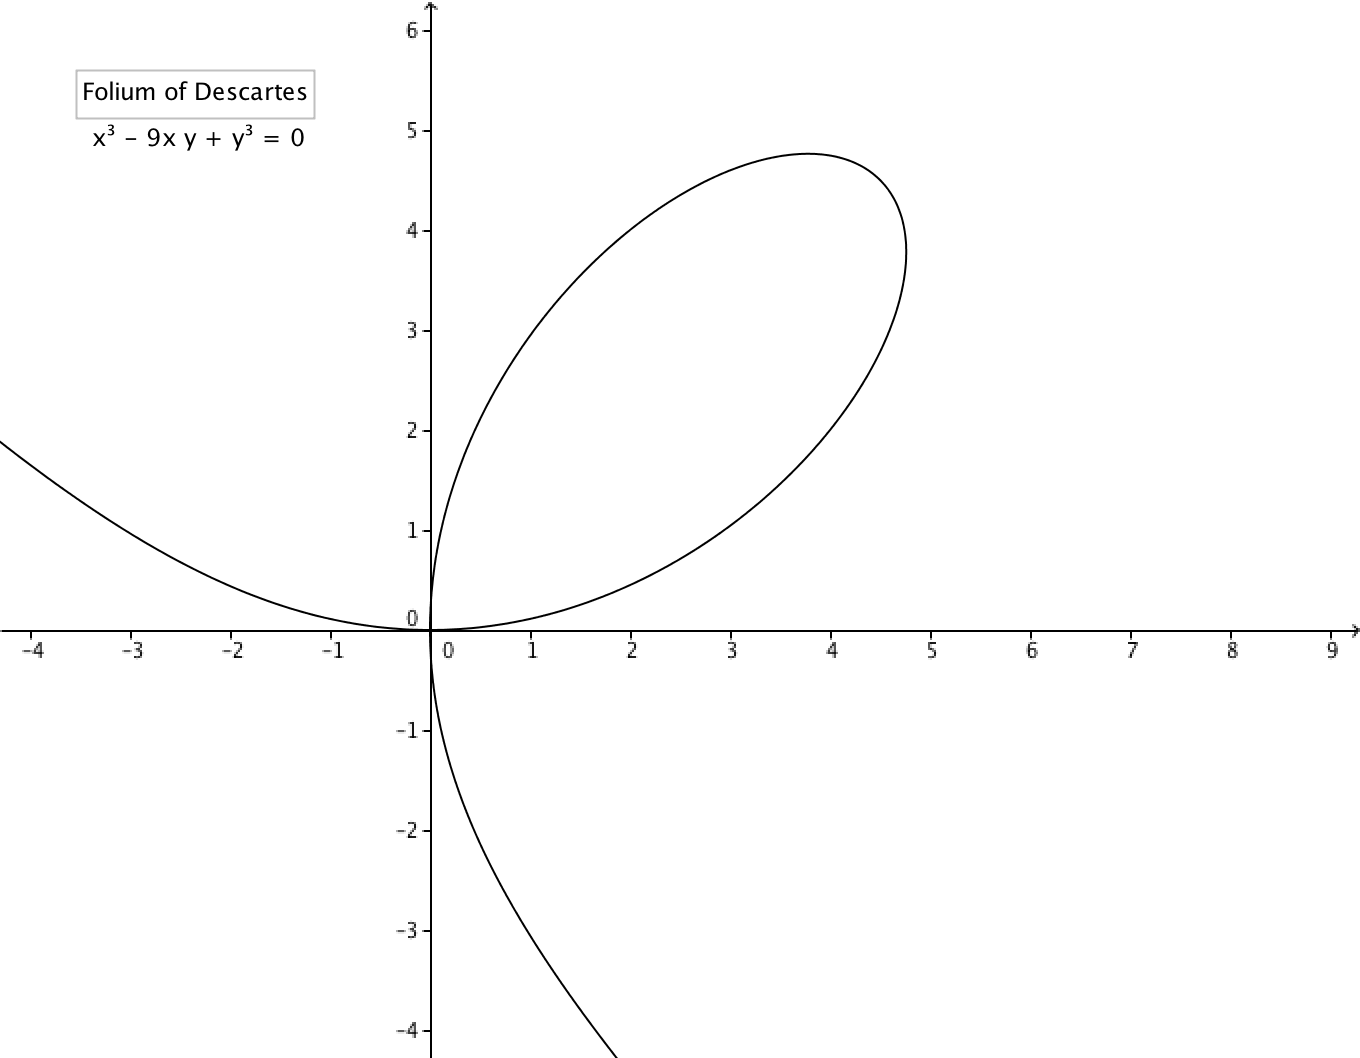
\includegraphics[width=2in]{middleCalculus/graphics/FoliumOfDescartes.png} \qquad
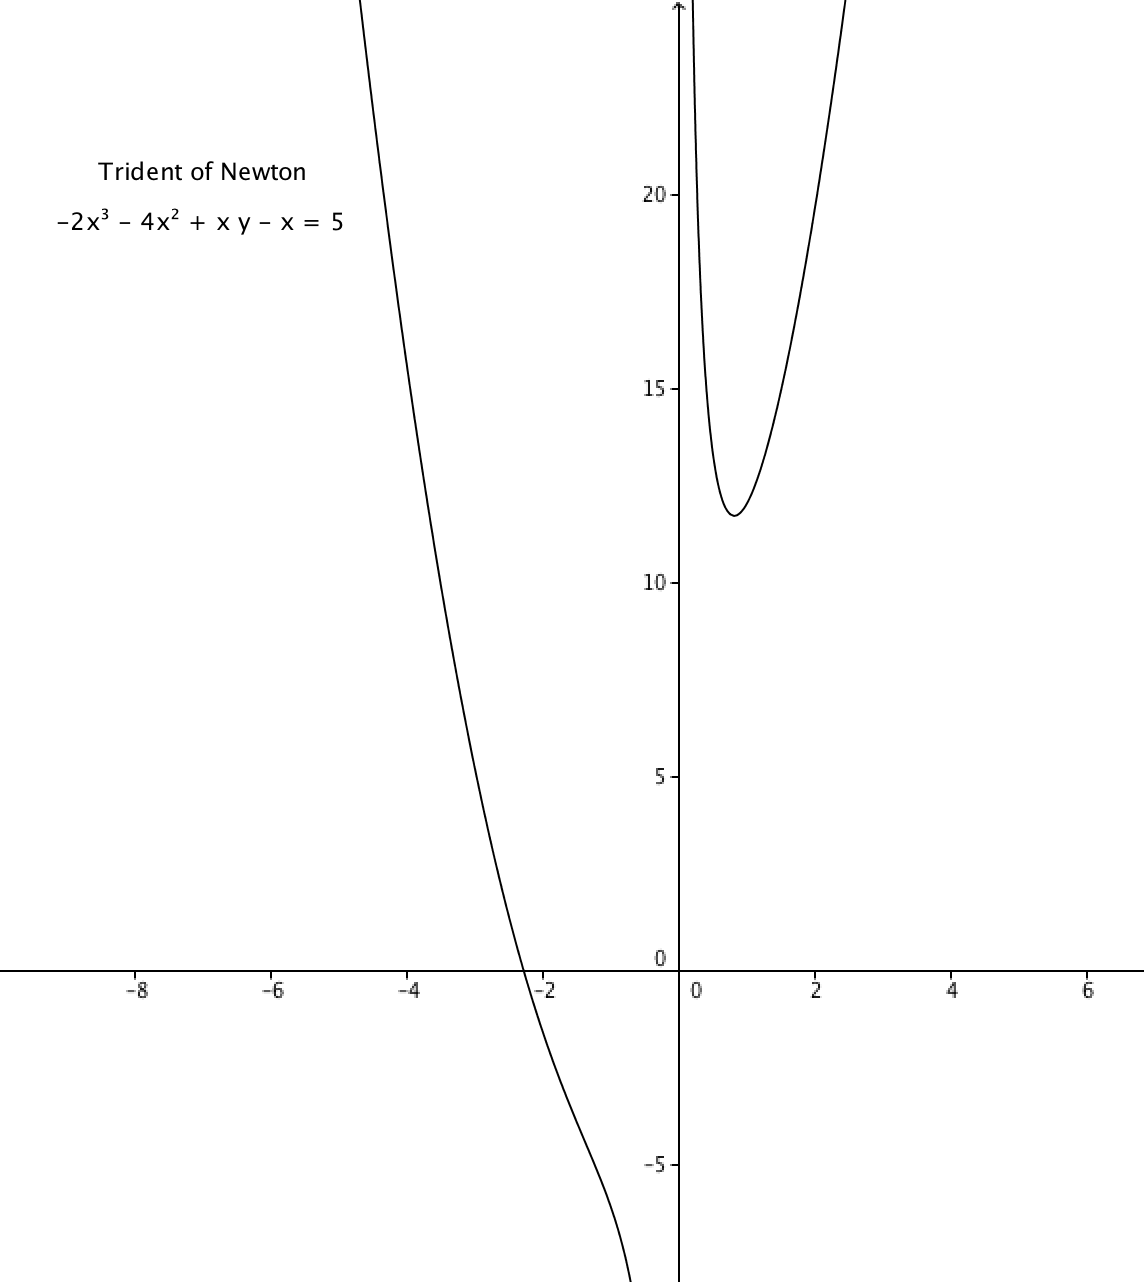
\includegraphics[width=2in]{middleCalculus/graphics/TridentOfNewton.png}
\]
\[
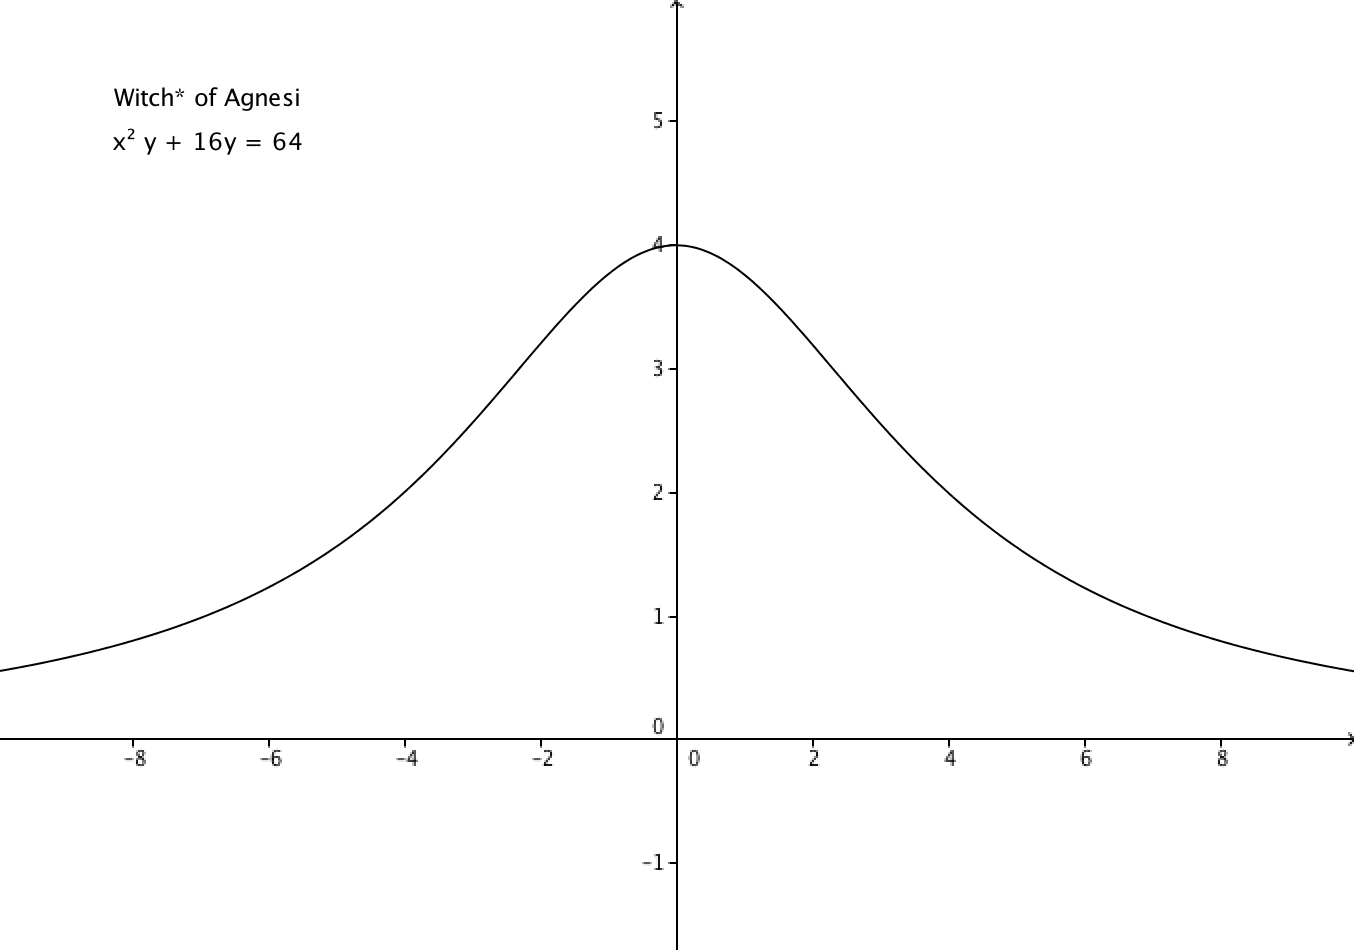
\includegraphics[width=2in]{middleCalculus/graphics/WitchOfAgnesi.png} \qquad
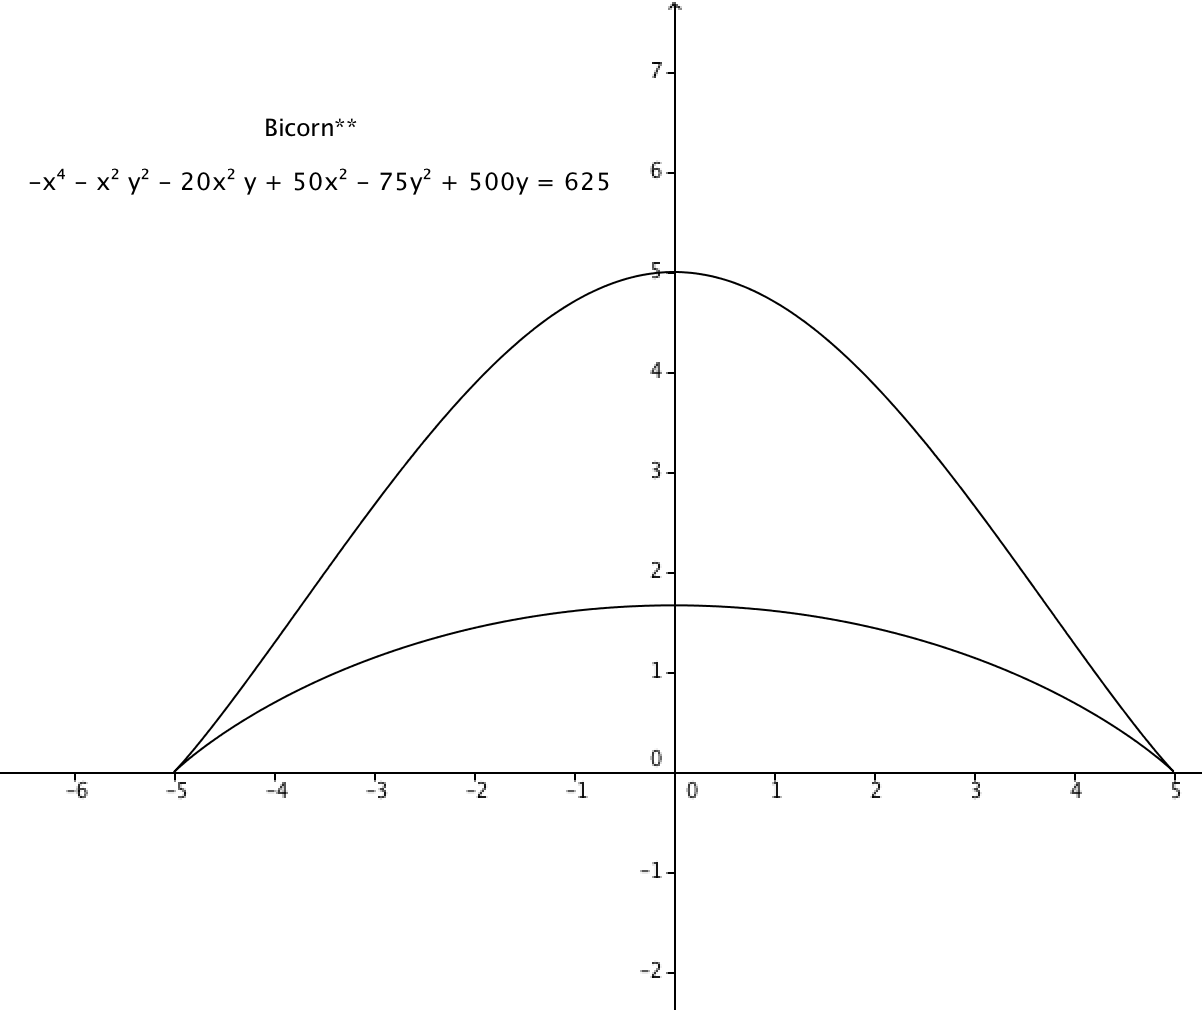
\includegraphics[width=2in]{middleCalculus/graphics/Bicorn.png}
\]

For more on each of these curves, check out the following links. \link[Folium of Descartes]{http://www-history.mcs.st-and.ac.uk/Curves/Foliumd.html}; \link[Trident of Newton]{http://www-history.mcs.st-and.ac.uk/Curves/Trident.html}; \link[Witch of Agnesi]{http://www-history.mcs.st-and.ac.uk/Curves/Witch.html}; \link[Bicorn]{http://www-history.mcs.st-and.ac.uk/Curves/Bicorn.html}

Now, we who live in Math 2167-land don't really care about these curves as curves in themselves, but we will be concerned about slopes to these curves.  To prepare for that, we, of course, ``cheat'', and pretend that $y$ is actually a function of $x$ (i.e., $y$ is the same as some $f(x)$).  Here are some warmup exercises:

\begin{exercise} 
Find the derivative with respect to $x$ of the following (Note: The left side is written with $y$ and the right side is written with $f(x)$.  Pick one of them ($y$ and $f(x)$ are the same thing) and, like in previous homeworks, take its derivative with respect to $x$):
\begin{enumerate}
    \item $\sqrt{y} = \sqrt{f(x)}$
    \item $e^y = e^{f(x)}$
    \item $\sin y = \sin f(x)$
    \item $x^3y^5 = x^3(f(x))^5$
    \item $x^3 (\cos y)^5 = x^3(\cos (f(x)))^5$
\end{enumerate}
\end{exercise}
        Now let’s find some slopes to these curves:
\begin{exercise} 
Show that the point $(-10,  \sqrt{44})$ is on the circle  $x^2 + y^2 = 144$.  Find the slope at that point.  Why does this slope make sense on the graph?
\end{exercise}
\begin{exercise} 
Show that the point $(2, 4)$ is on the Folium of Descartes  $x^3+y^3=9xy$.  Find the slope at that point.  Why does this slope make sense on the graph (shown above)?  What about the slope at $(4,2)$?
\end{exercise}



\end{document}